% Slides for 2024-08-20
\begin{frame}{Endpoint detection}
    \begin{enumerate}
        \item Estimate endpoints using PCA
        \item Classify as head/tail
        \item Use a separate heuristic for each to adjust
    \end{enumerate}
\end{frame}

\begin{frame}{Head/tail classification}
    \begin{columns}
        \begin{column}{0.7\textwidth}
            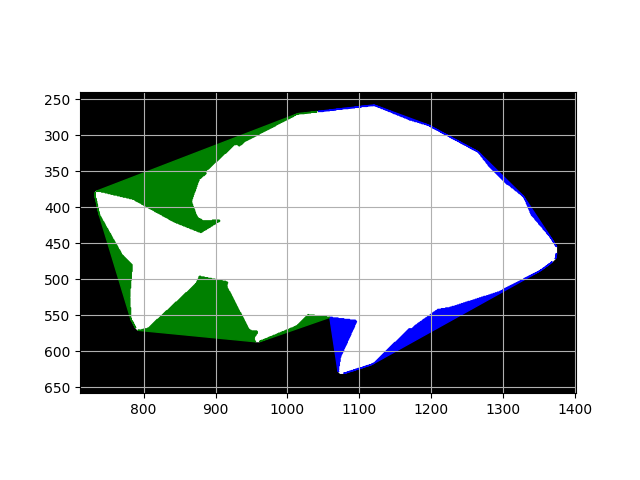
\includegraphics[height=0.7\textheight,width=0.7\textwidth,keepaspectratio]{images/fs_convex_difference.png}
        \end{column}
        \begin{column}{0.4\textwidth}

            \begin{itemize}
                \item Old alg: 125/138
                \item New alg: 138/138
                \item 100\%!
            \end{itemize}
        \end{column}
    \end{columns}
\end{frame}

\begin{frame}{Head point correction}
    \centering
    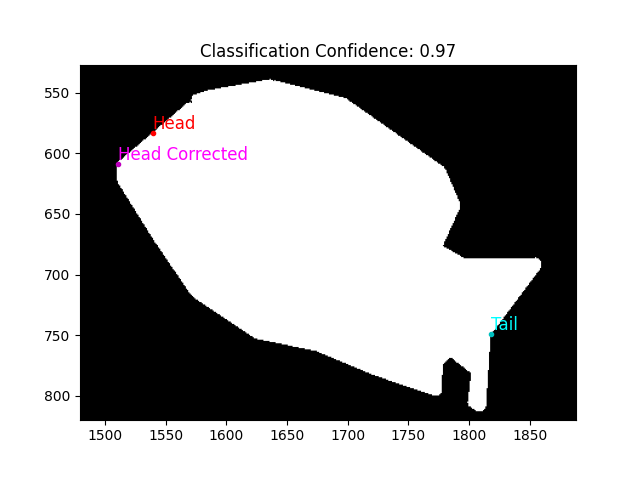
\includegraphics[height=0.6\textheight,width=0.6\textwidth,keepaspectratio]{images/fs_head_correction1.png}
    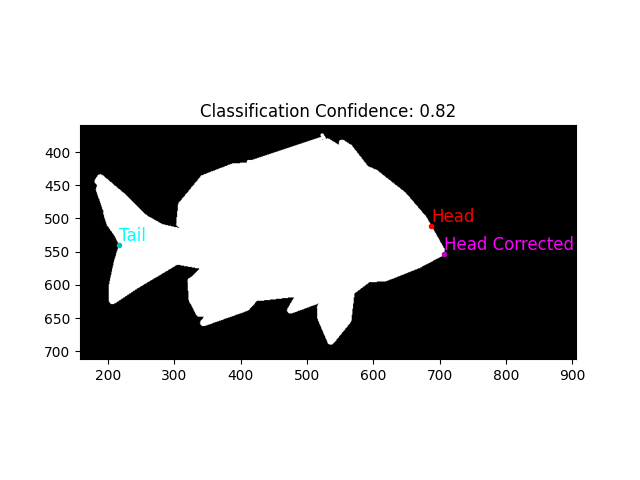
\includegraphics[height=0.6\textheight,width=0.6\textwidth,keepaspectratio]{images/fs_head_correction3.png}
\end{frame}

\begin{frame}{Head point correction}
    \centering
    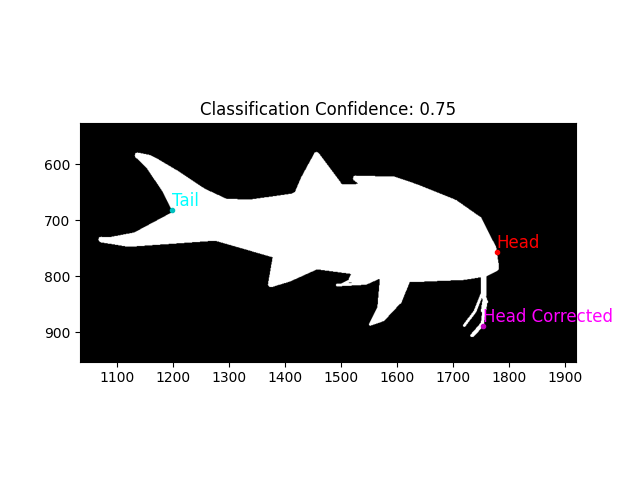
\includegraphics[height=0.6\textheight,width=0.6\textwidth,keepaspectratio]{images/fs_head_correction5.png}
    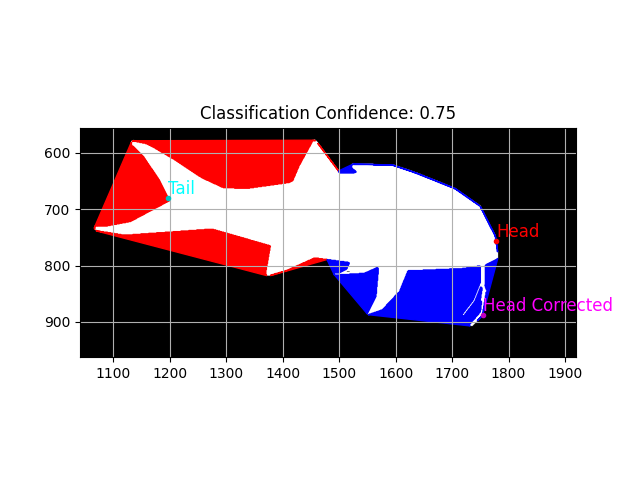
\includegraphics[height=0.6\textheight,width=0.6\textwidth,keepaspectratio]{images/fs_head_correction6.png}
\end{frame}

\begin{frame}{FishSense Mobile - Fixed IG}
    \begin{columns}
        \begin{column}{0.5\textwidth}
            \centering
            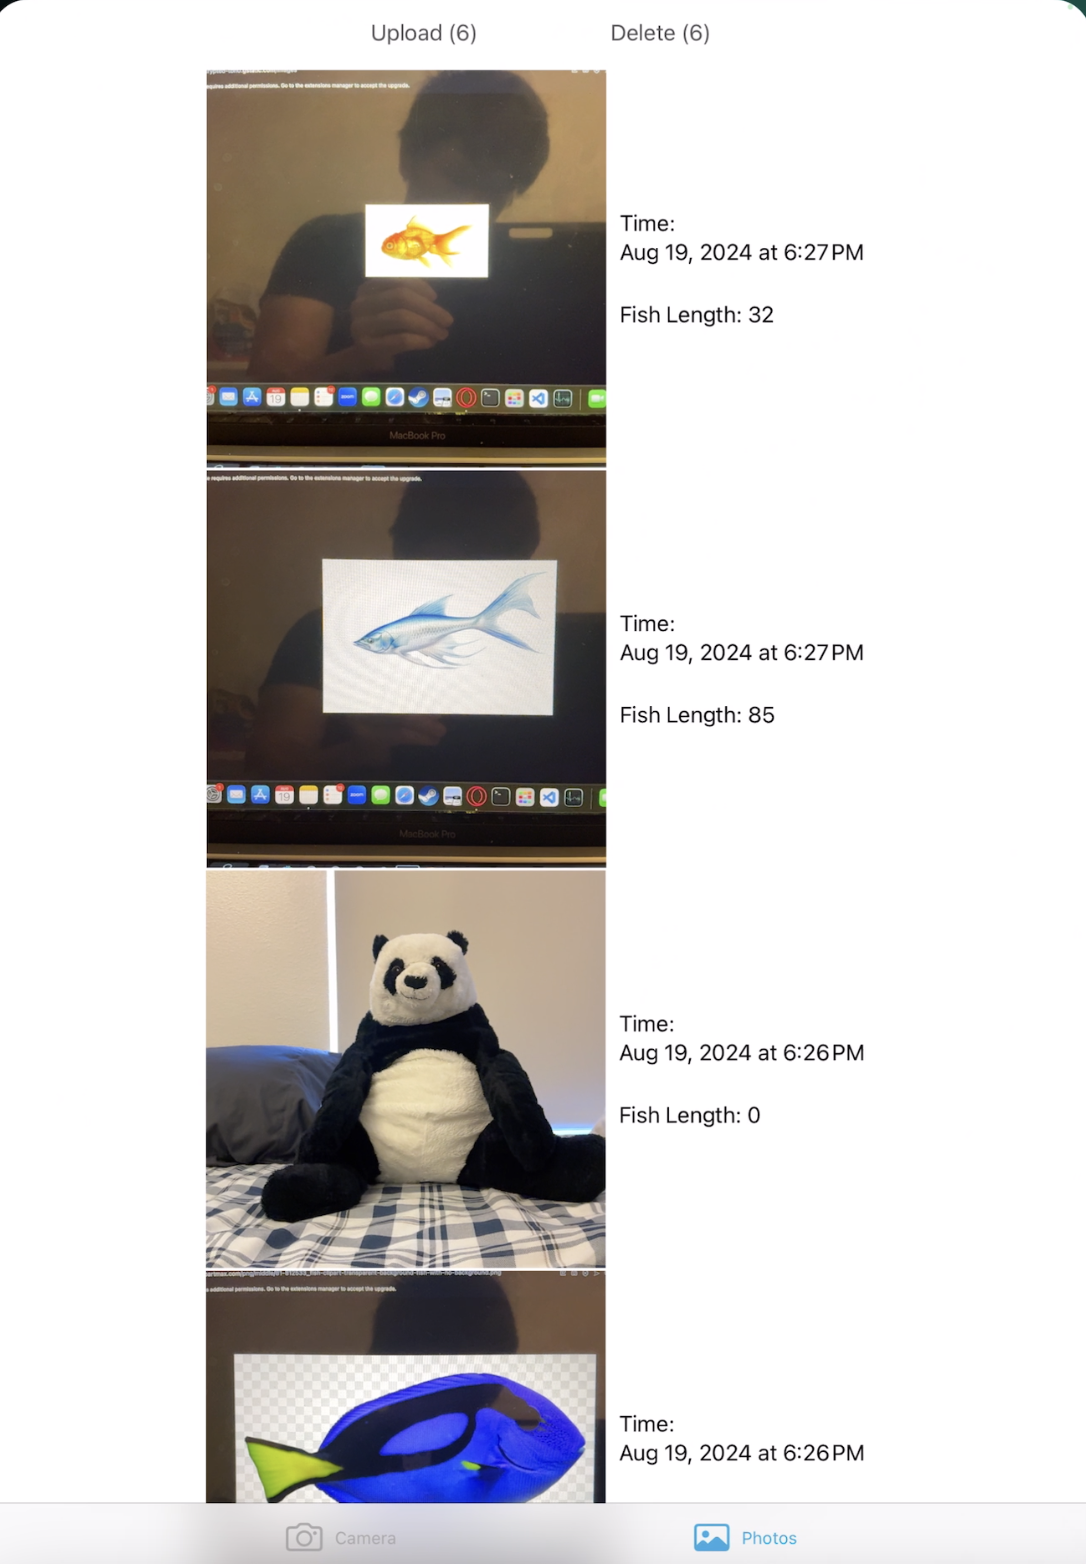
\includegraphics[height=0.8\textheight,width=0.7\textwidth,keepaspectratio]{images/fs_ipad1.png}
        \end{column}
        \begin{column}{0.5\textwidth}
            \centering
            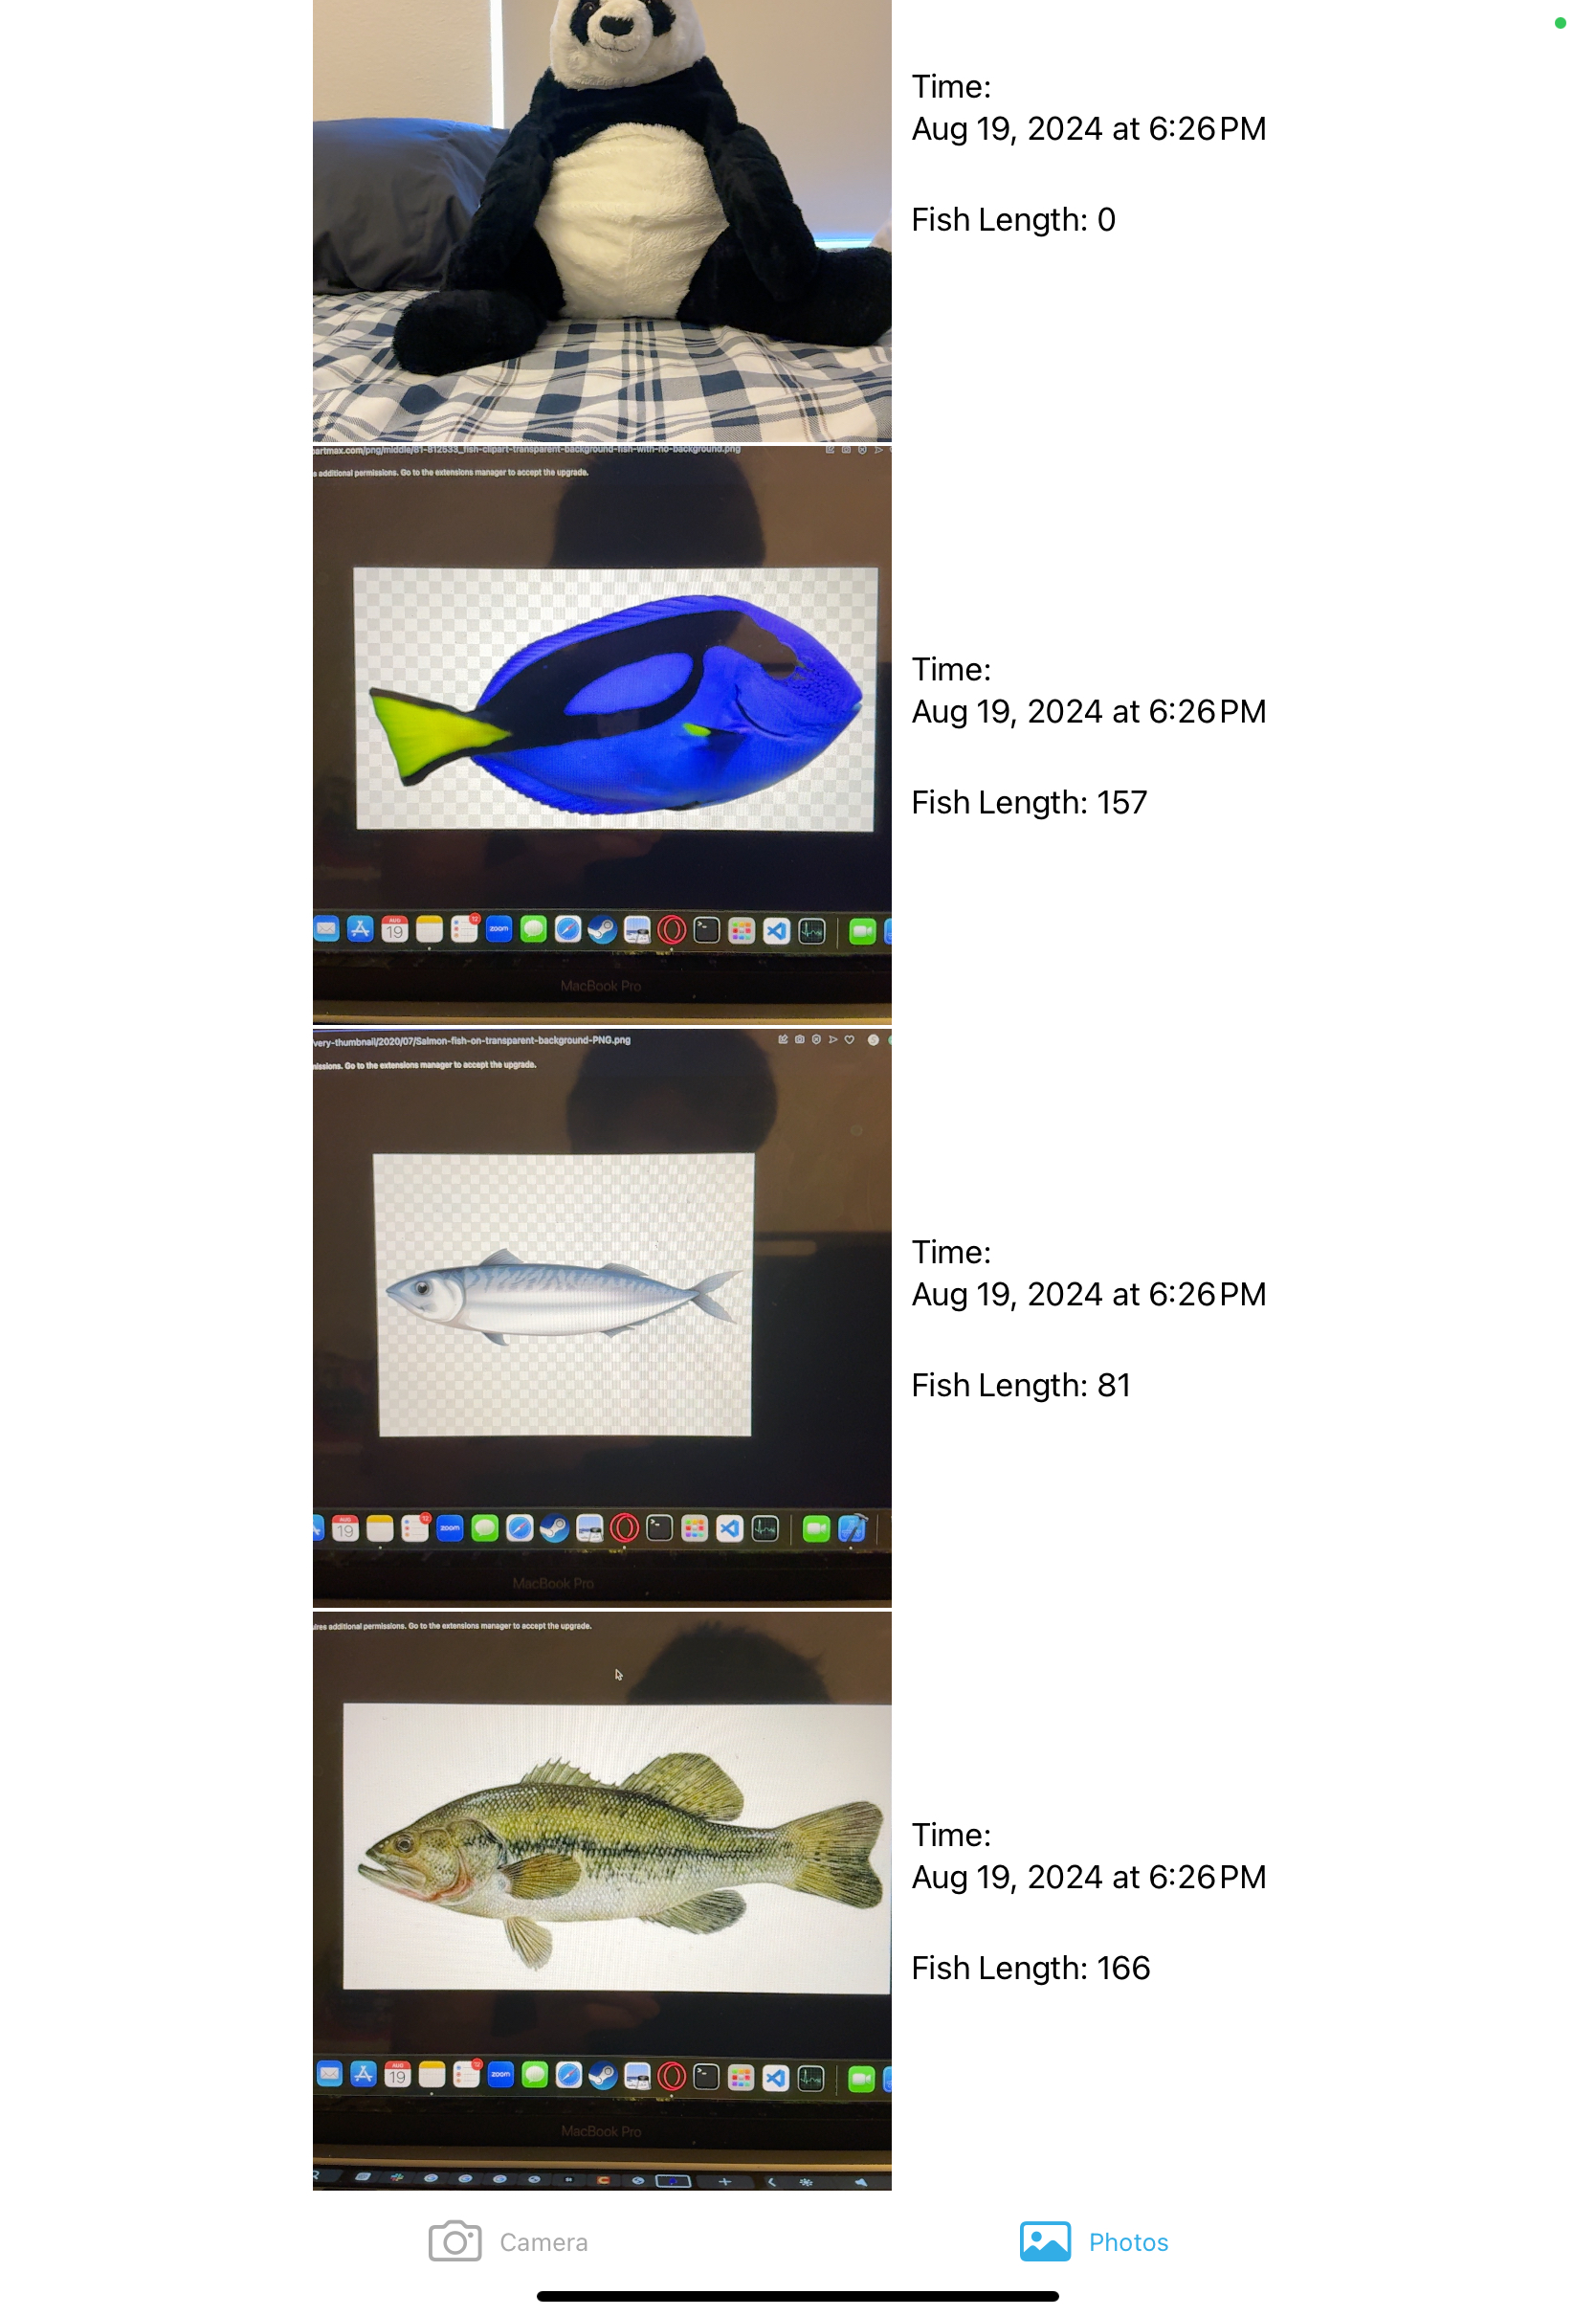
\includegraphics[height=0.8\textheight,width=0.7\textwidth,keepaspectratio]{images/fs_ipad2.jpeg}
        \end{column}
    \end{columns}
\end{frame}

\begin{frame}{FishSense Mobile - Delete}
    \centering
    \href{https://www.youtube.com/shorts/Q-dP97_H-QA}{Youtube Link}
\end{frame}


\begin{frame}{FishSense Segmentation}
    \centering
    \textbf{Finding in Fish Prompt Supervisor}
    \text{Depth-estimation method shows great capacity in separating foreground }
    \text{and background of a image, which helps to supervise ViT's encoding for SAM}
    \vspace{0.3cm} % Adjust space between title and images
    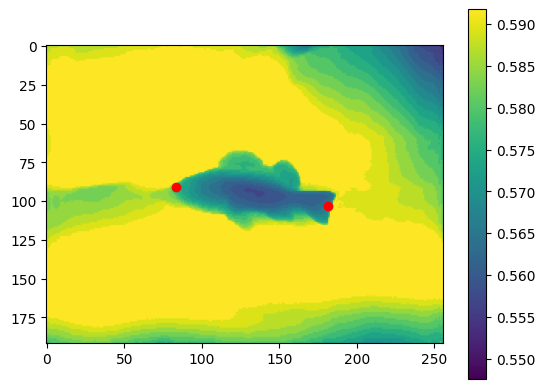
\includegraphics[width=\textwidth]{images/fs_depth_3.png}
    \vspace{0.3cm} % Adjust space between images and text

    \textit{Image enhancement helps very little for depth-based Supervisor}
\end{frame}


\begin{frame}{FishSense Segmentation}
    \centering
    \textbf{Finding in Fish Prompt Supervisor}

    \vspace{0.3cm} % Adjust space between title and images

    \begin{minipage}{0.48\textwidth}
        \centering
        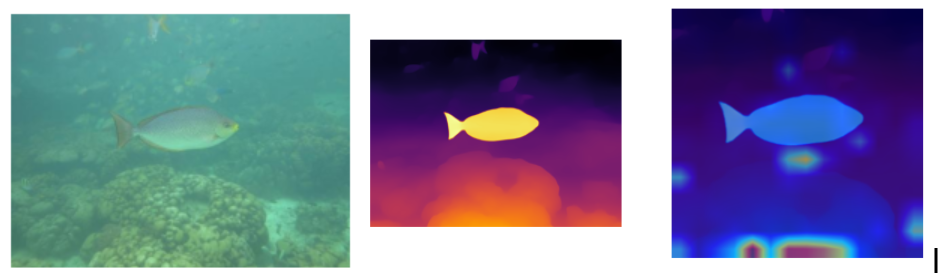
\includegraphics[width=\textwidth]{images/fs_depth_1.png}\\
        % Caption below each image (optional)
        % \small{Caption for first image}
    \end{minipage}
    \hfill
    \begin{minipage}{0.48\textwidth}
        \centering
        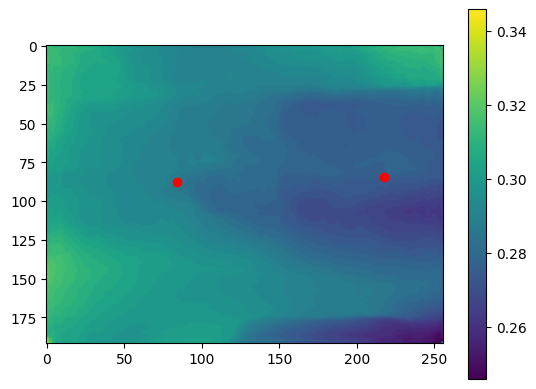
\includegraphics[width=\textwidth]{images/fs_depth_2.png}\\
        % Caption below each image (optional)
        % \small{Caption for second image}
    \end{minipage}

    \vspace{0.3cm} % Adjust space between images and text

    \textit{Image enhancement helps very little for depth-based Supervisor}
\end{frame}

\begin{frame}{FishSense Segmentation}
    \centering
    \textbf{Adjusted New Pipeline}

    \vspace{0.3cm} % Adjust space between title and image

    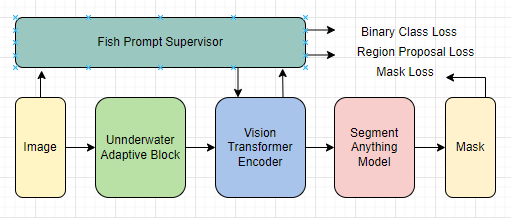
\includegraphics[width=0.85\textwidth,keepaspectratio]{images/fs_seg_pipeline4.png}
\end{frame}
